\section{Basics}
\subsection{Basics of Nuclear Magnetic Resonance}

Nuclear Magnetic Resonance techniques relay of the interaction between the magnetic dipole moment
\begin{equation}
\label{magnetic dipole moment}
\vec{\mu} = \hbar\gamma\vec{S} 
\end{equation}
 of nuclei with non-zero spin $S$ and an external magnetic field $\vec{B_0}$. In the following paper $\gamma$ represents the gyro-magnetic ratio of protons:
 \begin{equation}
 \label{gamma proton}
 \gamma_{proton} = 2.6752 \cdot 10^8 \, \textrm{sec}^{-1}\textrm{Tesla}^{-1}.
 \end{equation}
The resulting interaction energy, also called spin-lattice contribution, is defines as:
\begin{equation}
\label{interaction energy}
\Delta E = -\vec{\mu}\cdot\vec{B}_0.
\end{equation}

In a classical description, this interaction yields two states for the orientation of the protons's magnetic dipole in the external magnetic field: $\mu_+$ (parallel) and $\mu_-$ (antiparalle).
For a macroscopic sample of $N$ protons, both numbers of occupied states $N_+$ and $N_-$, the sum of which comprises $N$, can be approximated by a Boltzmann distribution:
\begin{equation}
\label{ocupation number}
 N_\pm = N_0e^{-\frac{E_0\pm\Delta E}{kt}}
\end{equation}
with $N_0$ as a normalization factor. However $N_+ > N_-$, since the parallel state is energetically favorale. The predominance of protons in the parallel state leads to a macroscopic magnetization, whose ground state is
\begin{equation}
\label{magnetization ground state}
\vec{M}_0 = \frac{\mu N}{V}\sinh{\left(\frac{\mu B}{kT}\right)} \vec{e}_z .
\end{equation}
In our case, a weak field ($\mu B \gg kT$), the former expression simplifies to
\begin{equation}
\label{ground state approx}
\vec{M}_0 = \frac{N}{V} \frac{\hbar^2 \gamma^2 I(I+1)}{3kT}\vec{B}_0 \propto \frac{\vec{B}_0}{T},
\end{equation}
i.e the law of Curie.

In general, the magnetization can have an arbitrary orientation related to the external magnetic field, however such a system will decay asymptotically into the ground state, since $\vec{M}_0$ minimizes the energy. 

The interaction between the macroscopic magnetization and the external magnetic field result in a torque
\begin{equation}
\vec{\tau} = \gamma\vec{M} \wedge\vec{B}_0.
\end{equation}
If the magnetization is separated into parallel $\vec{M}_{\parallel}$ and perpendicular $\vec{M}_{\perp}$ components, relative to the external field, we quickly see that only the later gives a none trivial expression. Without any relaxation processes, the rate of change of the former is given by
\begin{equation}
\frac{d \vec{M}_{\perp}}{dt} = -\vec{M}_{\perp}\wedge\vec{B}_0.
\end{equation}
The last equation describes the precession of $\vec{M}_{\perp}$ around $\vec{B}_0$. The angular frequency of this process is called Larmor frequency
\begin{equation}
\omega_L = \gamma B_0.
\end{equation}

Generating a transverse or anti-parallel magnetization to $\vec{B}_0$ can be achieved by applying a high frequency pulse to the ground state magnetization $\vec{M}_0$. 
Let the static magnetic field $\vec{B}_0$ be pointing in z-direction. Now consider a coil oriented along the x-axis, if a sinusoidal voltage with frequency $\omega_H$ is applied it would generate a solenoid magnetic field $\vec{B}_1(t)$ polarized along the x-direction. Under this conditions the torque  acquires a second term:
\begin{equation}
\vec{\tau} = \vec{M}_0\wedge(\vec{B}_0 + \vec{B}_1(t)
\end{equation}
which induces a second precession around the x-axis.
For pulse duration which are short relative to the relaxation times, the magnitude of the magnetization is approximately constant. In this case the vector $\vec{M}$ moves in a sphere with radius $|\vec{M}_0|$. The vector coordinates in the sphere are then given by a azimuthal angle $\varphi$ which is defined by the precession induced by $\vec{B}_0$, and by a polar angle $\theta$ which arise from interaction with the solenoid field. Both angles are a functions of time:
\begin{equation}
\varphi = \omega_L t
\end{equation}
\begin{equation}
\theta = \gamma B_1 t.
\end{equation}

A pulse which induces a  polar angle $\theta = 90$° is called a 90° pulse. For such a pulse the ground state magnetization is transformed into transverse magnetization $\vec{M}_{\perp}$, with $\vec{M}_{\parallel} = 0$. Analogously a pulse which generates $\theta = 180°$ is called a 180° pulse. Such a pulse transforms the ground state into an anti-parallel magnetization $\vec{M}_{\perp} = -\vec{M}_0$, with $\vec{M}_{\parallel} = 0$.
\subsection{NMR signal}
\subsubsection{Signal generation}
In the set up used for this experiment the high frequency pulses of fixed frequency $\omega_{HF} = 19.8$ MHz were generated in a electronic unit of the minispec p20. Said pulses induce a precession around de z-axis, as explain in the previous section, that change the magnetic flux through the coil in time resulting in a induction signal modulated by the Larmor frequency $\omega_L$, which could be set up by hand. This signal is fed back to the p20 electronic unit, where both the high frequency and the induction signals are mixed into an output given by the multiplication of both inputs, i.g the sum of two cosine functions. One of the terms depends on the working frequency, which is given by the difference between $\omega_L$ and $\omega_{HF}$, and is on the order of few hundred Hertz while the second one in the range of 40MHz. The use of a low frequency bandpass filter allows to get rid of the former signal.   
\subsection{Relaxation Time}
\subsubsection{Bloch equations}
For the description of the precession of $\vec{M}_{\perp}$ it is possible to define a rotating reference system $(x', y', z)$. This reference frame is defined by 2 condition: 1) the $(x', y')$-plane rotate in the static $(x, y)$-plane and 2) $\vec{M}_{\perp}$ points in the $x'$-direction.

In this reference system the transverse and longitudinal magnetizations are constant if no relaxations processes are present, otherwise both components are time dependent. Their time evolution is described by the Bloch equations:
\begin{equation}
\label{eq: bloch T2}
\frac{d\vec{M}_\perp^{rot}}{dt} = -\frac{\vec{M}_\perp^{rot}}{T_2}
\end{equation}
\begin{equation}
\label{eq: bloch T3}
\frac{d\vec{M}_\parallel^{rot}}{dt} = -\frac{\vec{M}_\parallel^{rot} - \vec{M}^{rot}}{T_1}.
\end{equation}
In the later equations it is assumed that the time evolution is dominated by a restoring force which is linearly proportional to the deflection from equilibrium. The constant $T_2$ in \ref{eq: bloch T2} is the so called spin-spin relaxation time whereas $T_1$ in \ref{eq: bloch T3} is called the spin-lattice relaxation time. The ground state is equal in the rotating and the static reference frame. 

In the presence of relaxation processed the time evolution of the magnetization in laboratory $\vec{M}$ and in rotating system $\vec{M}^{rot}$ are related by 
\begin{equation}
 \frac{d \vec{M}}{dt} = \frac{\partial \vec{M}^{rot}}{\partial t} + \vec{\omega}\wedge\vec{M}
 \end{equation}
 given the following Bloch equations in laboratory system:
 \begin{equation}
 \label{bloch + rot T2}
   \frac{d \vec{M}_{\perp}(t)}{dt} = \gamma(\vec{B}\wedge\vec{M})_\perp - \frac{\vec{M}_\perp (T)}{T_2},
  \end{equation} 
  \begin{equation}
  \label{bloch + rot T1}
     \frac{d \vec{M}_{\parallel}(t)}{dt} = \gamma(\vec{B}\wedge\vec{M})_\parallel  -\frac{\vec{M}_\parallel (t)-\vec{M}_0}{T_1}.
  \end{equation}
 \subsubsection{Spin-spin relaxation $T_2$}
The magnetic field that interacts with the magnetization is not constant, firstly due to possible variations of the applied static field, but more important due to the magnetic interactions between the sample's protons with themselves which can generate slowly varying field inhomogeneities. Furthermore, thermally induced rotations as well as translations of nuclei, caused by molecular diffusion, throughout spatially varying magnetic environments will causes the field that any nucleus experiences to be time-dependent. This inhomogeneities caused the protons at different positions to precess with different frequencies which induces a dephasing and therefore a decay of the magnetization, i.g the magnetization undergoes a relaxation process called the spin-spin relaxation characterized by the relaxation time $T_2$. Said decay is described by the solution of \ref{bloch + rot T2}:
\begin{equation}
\vec{M}_{\perp}(t)= \vec{M}_\perp^{0}\exp^{-\frac{t}{T_2}}.
\end{equation}
In the following experiment two different methods were used to measure $T_2$: 1) spin-echo/ Hahn echo method and 2) Carr-Purcell sequence. In both cases a 180° pulse is used to reverse the dephasing. 
\paragraph{Spin-Echo:}
A)We start with a system in the ground state.B) At $t = 0$ a 90° pulse induce a transverse magnetization, which precess in clockwise fashion around the z-axis. Consider that at location $A$ the applied magnetic field is strong than at location $B$, hence $\omega_A > \omega_B$. C) At $t = \tau$ the spin-spin-relaxatiton has induce a dephasing of protons at location $A$ and $B$, i.g the protons that were at position $A$ are ahead of the ones with frequency $\omega_B$. At this moment a 180° pulse is applied which rotates the orientation of the protons' dipoles by 180° around x-axis. D) After the pulse the configuration is reversed, the "fast protons" with frequency $\omega_A$ are behind "slow ones". E) After this transformation all particles keep on rotating clockwise, such that at $t = 2\tau$ they are in phase again, F). The process is illustrated in Fig. \ref{fig: spin-echo}. 
\begin{figure}[!htbp]
 \begin{center}
  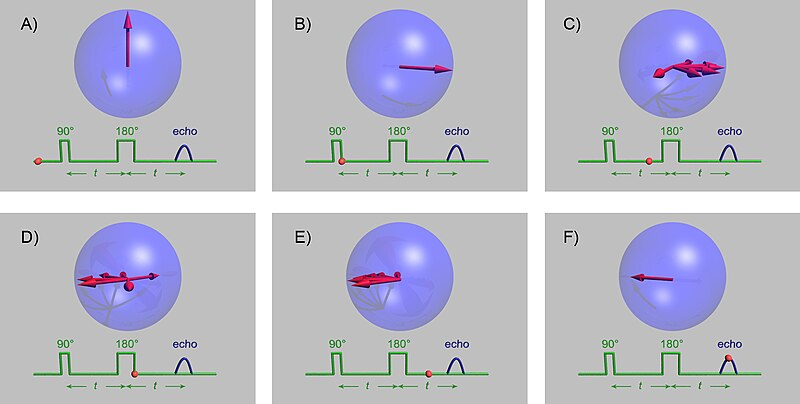
\includegraphics[width = .8\textwidth]{/Users/notchok/Documents/5. Semester/FP/FP/F61/Latex images/SpinEcho_GWM_stills.jpg}
  \caption[]{Spin-echo by a 90-180 sequence  \footnotemark}
    \label{fig: spin-echo}
 \end{center}
\end{figure}
\footnotetext{Nuclear magnetic resonance. (2024, May 16). \href{Wikipedia. https://en.wikipedia.org&/wiki/Nuclear_magnetic_resonance}{Quelle: wikipedia.org}}
The resulting signal is represented in Fig. \ref{fig: spin-echo signal}. There the decay of $\vec{M}_\perp$ is visible at time $t<5$ ms and the spin echo is to be seeing in the time range $15$ ms < $t$ < $25$ ms.
\begin{figure}[!htbp]
 \begin{center}
  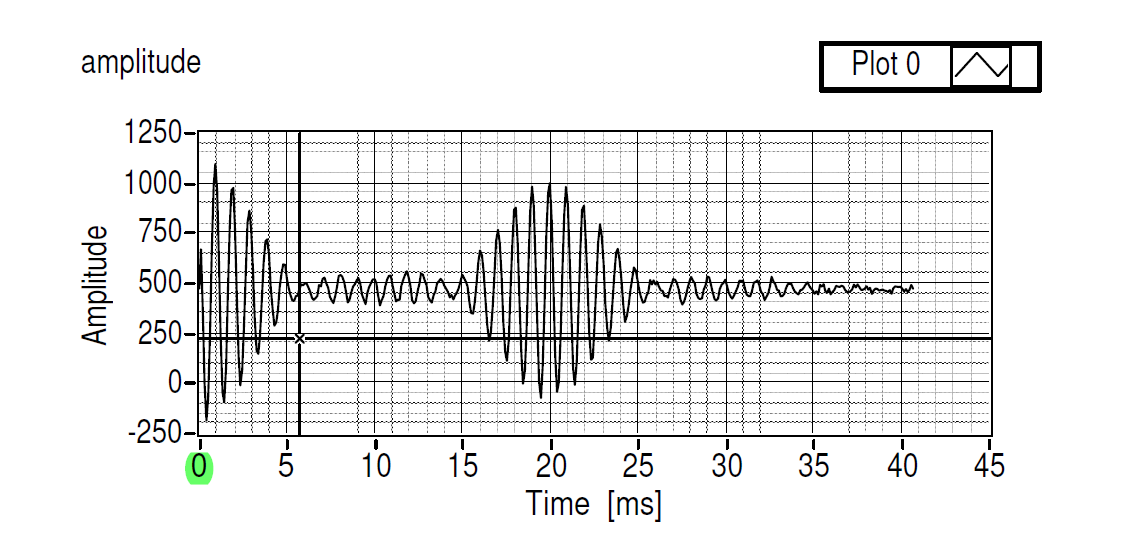
\includegraphics[width = .8\textwidth]{/Users/notchok/Documents/5. Semester/FP/FP/F61/Latex images/spin_echo_signal.png}
  \caption[]{Spin-echo by a 90-180 sequence  \footnotemark}
    \label{fig: spin-echo signal}
 \end{center}
\end{figure}
\footnotetext{R. Schicker (2021, March 4). Nuclear Magnetic Resonance F61/F62 p. 13} 
Due to Parseval's theorem it is possible to estimate the signal's strength by calculating the are under the spin-echo curvature in frequency space, which is given by a Gaussian profile. The decay curve of \ref{bloch + rot T2} is measured by varying the parameter $\tau$ in the 90-180 sequence.

The Hahn echo finds its limitations when measuring the decay curvature for large $t$. For this cases the system 
\subsection{Chemical shift}
\subsection{Imagin with NMR}
